\begin{figure}[tbp]
  \centering
  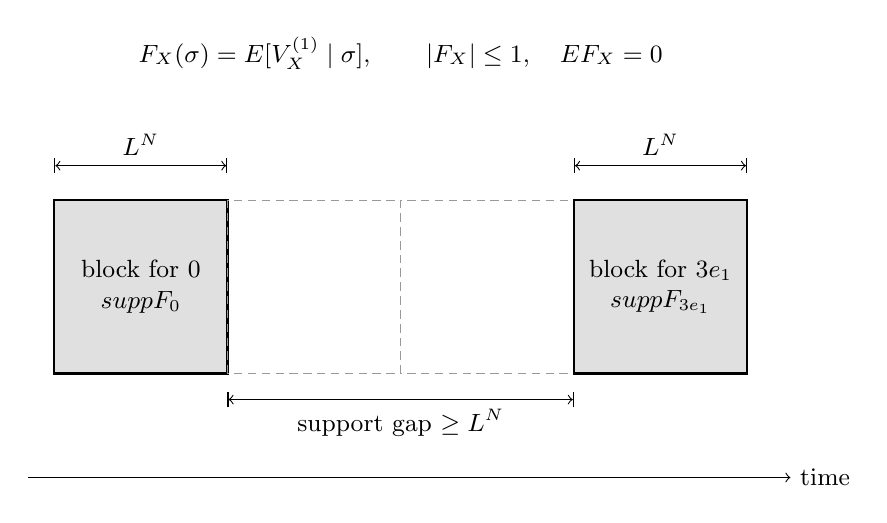
\begin{tikzpicture}[x=2.2cm,y=2.2cm,font=\small]
    \draw[fill=black!12,thick] (0,0) rectangle (1,1);
    \draw[densely dashed,black!40] (1,0) rectangle (2,1);
    \draw[densely dashed,black!40] (2,0) rectangle (3,1);
    \draw[fill=black!12,thick] (3,0) rectangle (4,1);
    \node[align=center] at (0.5,0.5) {block for $0$\\$\operatorname{supp} F_0$};
    \node[align=center] at (3.5,0.5)
      {block for $3e_1$\\$\operatorname{supp} F_{3e_1}$};

    \draw[|<->|] (0,1.2) -- (1,1.2);
    \node[above] at (0.5,1.2) {$L^N$};
    \draw[|<->|] (3,1.2) -- (4,1.2);
    \node[above] at (3.5,1.2) {$L^N$};
    \draw[|<->|] (1,-0.15) -- (3,-0.15);
    \node[below] at (2,-0.15) {support gap $\ge L^N$};
    \draw[->] (-0.15,-0.6) -- (4.25,-0.6);
    \node[anchor=west] at (4.25,-0.6) {time};

    \node at (2,1.85)
      {$\displaystyle F_X(\sigma)=\mathbb E[V_X^{(1)}\mid\sigma],
       \qquad |F_X|\le1,\quad \mathbb E F_X=0$};
  \end{tikzpicture}\par\medskip
  \caption{Pulling terminal observables back to the original lattice.
  Each displayed support lies within an ancestral block of side $L^N$.
  The auxiliary block variables are independent between disjoint
  ancestral blocks conditional on the original spins, so
  $\mathbb E[F_0F_{3e_1}]=\mathbb E[V_0^{(1)}V_{3e_1}^{(1)}]$.
  Alignment bounds this correlation below by $1/8$; the full transfer
  gap bounds it above by the exponential of minus the gap times $L^N$.
  No independence of the two pulled-back observables is asserted.}
  \label{fig:block-supports}
\end{figure}
